\documentclass[11pt,a4paper]{article}
\usepackage[utf8]{inputenc}
\usepackage[margin=0.85in]{geometry}
\usepackage{amsmath,amssymb}
\usepackage{booktabs}
\usepackage{xcolor}
\usepackage{tabularx}
\usepackage{tikz}
\usetikzlibrary{shapes.geometric, arrows.meta, positioning, calc, fit, backgrounds}
\usepackage{hyperref}

% Define color palette
\definecolor{primaryblue}{RGB}{37, 99, 235}
\definecolor{accentemerald}{RGB}{16, 185, 129}
\definecolor{amberorange}{RGB}{245, 158, 11}
\definecolor{roseaccent}{RGB}{225, 29, 72}
\definecolor{darkslate}{RGB}{30, 41, 59}
\definecolor{cardbg}{RGB}{248, 250, 252}
\definecolor{bordergray}{RGB}{203, 213, 225}

\hypersetup{
    colorlinks=true,
    linkcolor=primaryblue,
    urlcolor=primaryblue,
    citecolor=primaryblue
}

\title{\textbf{GridWise EMS: Autonomous Campus Microgrid Dispatch Engine}\\[0.4ex]
\large System Architecture, Mathematical Model, and Scalability Report}
\author{\textbf{BUP CSE FEST 2026 Hackathon} --- Online Preliminary Round}
\date{September 2026}

\begin{document}

\maketitle

\begin{abstract}
This report details the architectural design, mathematical optimization formulation, and multi-tier resilience mechanisms of \textbf{GridWise EMS}. The platform solves the 24-hour campus microgrid energy dispatch problem under Time-of-Use (ToU) electricity tariffs and rooftop solar generation, translating unstructured operator shift notes into exact linear constraints via a multi-provider Large Language Model (LLM) cognitive pipeline. Directives are validated through deterministic guardrails and optimized via a pure-Rust Simplex Linear Programming (LP) solver executing in under 5 milliseconds with guaranteed physical invariant compliance.
\end{abstract}

\vspace{1em}

\section{System Architecture Diagram}

Figure~\ref{fig:architecture} illustrates the end-to-end processing pipeline, showing data flow from operator input ingestion to invariant-verified dispatch scheduling.

\begin{figure}[htbp]
\centering
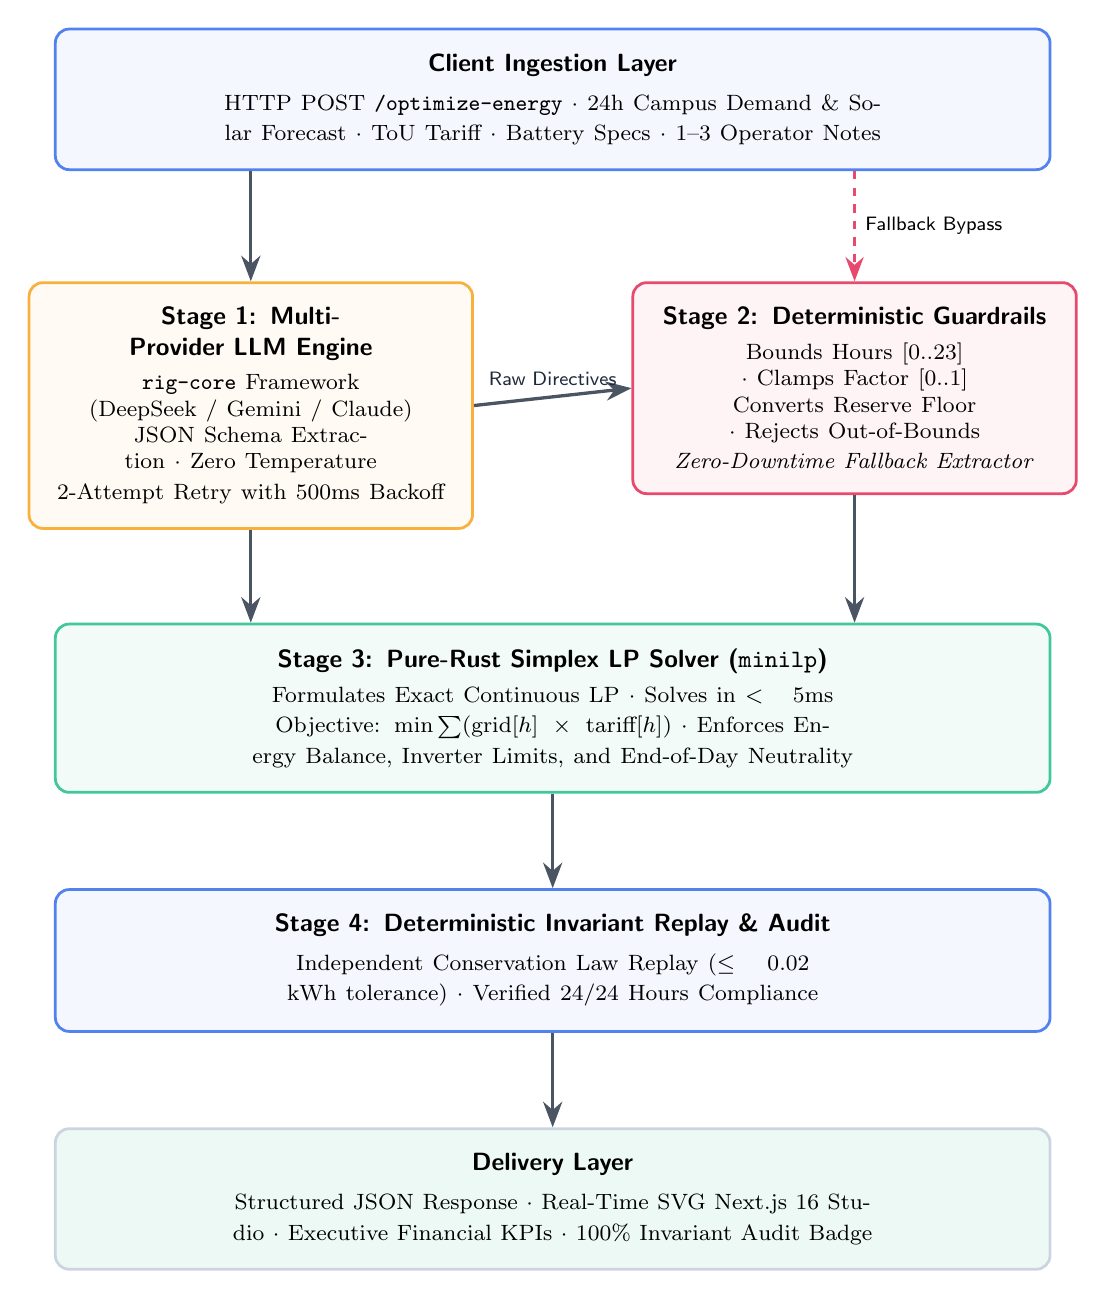
\begin{tikzpicture}[
    node distance=1.3cm,
    box/.style={
        rectangle,
        rounded corners=5pt,
        draw=bordergray,
        line width=1pt,
        fill=cardbg,
        inner sep=9pt,
        align=center,
        font=\small\sffamily
    },
    primarybox/.style={
        box,
        draw=primaryblue!80,
        fill=primaryblue!5,
        font=\small\sffamily\bfseries
    },
    solverbox/.style={
        box,
        draw=accentemerald!80,
        fill=accentemerald!5,
        font=\small\sffamily\bfseries
    },
    llmbox/.style={
        box,
        draw=amberorange!80,
        fill=amberorange!5,
        font=\small\sffamily\bfseries
    },
    guardbox/.style={
        box,
        draw=roseaccent!80,
        fill=roseaccent!5,
        font=\small\sffamily\bfseries
    },
    arrow/.style={
        -{Stealth[scale=1.1]},
        line width=1.2pt,
        draw=darkslate!80
    },
    dasharrow/.style={
        -{Stealth[scale=1.1]},
        dashed,
        line width=1.1pt,
        draw=roseaccent!80
    }
]

    % Top Layer: Client & Input
    \node[primarybox, text width=12cm] (client) at (0,0) {
        \textbf{Client Ingestion Layer} \\[3pt]
        \normalfont\footnotesize HTTP POST \texttt{/optimize-energy} $\cdot$ 24h Campus Demand \& Solar Forecast $\cdot$ ToU Tariff $\cdot$ Battery Specs $\cdot$ 1--3 Operator Notes
    };

    % Middle Layer - Left: LLM Engine
    \node[llmbox, text width=5cm, anchor=north east] (llm) at ([xshift=-1cm, yshift=-1.4cm]client.south) {
        \textbf{Stage 1: Multi-Provider LLM Engine} \\[3pt]
        \normalfont\footnotesize \texttt{rig-core} Framework (DeepSeek / Gemini / Claude) \\
        JSON Schema Extraction $\cdot$ Zero Temperature \\
        2-Attempt Retry with 500ms Backoff
    };

    % Middle Layer - Right: Guardrails & Fallback
    \node[guardbox, text width=5cm, anchor=north west] (guard) at ([xshift=1cm, yshift=-1.4cm]client.south) {
        \textbf{Stage 2: Deterministic Guardrails} \\[3pt]
        \normalfont\footnotesize Bounds Hours $[0..23]$ $\cdot$ Clamps Factor $[0..1]$ \\
        Converts Reserve Floor $\cdot$ Rejects Out-of-Bounds \\
        \textit{Zero-Downtime Fallback Extractor}
    };

    % Solver Layer
    \node[solverbox, text width=12cm, below=1.4cm of $(llm.south)!0.5!(guard.south)$] (solver) {
        \textbf{Stage 3: Pure-Rust Simplex LP Solver (\texttt{minilp})} \\[3pt]
        \normalfont\footnotesize Formulates Exact Continuous LP $\cdot$ Solves in $<5$ms \\
        Objective: $\min \sum (\text{grid}[h] \times \text{tariff}[h])$ $\cdot$ Enforces Energy Balance, Inverter Limits, and End-of-Day Neutrality
    };

    % Audit & Verification Layer
    \node[primarybox, text width=12cm, below=1.2cm of solver] (audit) {
        \textbf{Stage 4: Deterministic Invariant Replay \& Audit} \\[3pt]
        \normalfont\footnotesize Independent Conservation Law Replay ($\le 0.02$ kWh tolerance) $\cdot$ Verified 24/24 Hours Compliance
    };

    % Output Layer
    \node[box, text width=12cm, fill=accentemerald!8, below=1.2cm of audit] (output) {
        \textbf{Delivery Layer} \\[3pt]
        \normalfont\footnotesize Structured JSON Response $\cdot$ Real-Time SVG Next.js 16 Studio $\cdot$ Executive Financial KPIs $\cdot$ 100\% Invariant Audit Badge
    };

    % Arrows
    \draw[arrow] (client.south -| llm.north) -- (llm.north);
    \draw[arrow] (llm.east) -- node[above, font=\scriptsize\sffamily, text=darkslate] {Raw Directives} (guard.west);
    \draw[dasharrow] (client.south -| guard.north) -- node[right, font=\scriptsize\sffamily] {Fallback Bypass} (guard.north);
    \draw[arrow] (guard.south) -- (guard.south |- solver.north);
    \draw[arrow] (llm.south) -- (llm.south |- solver.north);
    \draw[arrow] (solver.south) -- (audit.north);
    \draw[arrow] (audit.south) -- (output.north);

\end{tikzpicture}
\caption{GridWise EMS 4-stage autonomous cognitive optimization pipeline.}
\label{fig:architecture}
\end{figure}

\section{Mathematical Optimization Formulation}

The continuous optimization engine solves an exact Linear Program over $h \in \{0, 1, \dots, 23\}$:

\subsection{Objective Function}
\begin{equation}
\min \sum_{h=0}^{23} \text{grid\_kwh}[h] \times \text{tariff\_bdt\_per\_kwh}[h]
\end{equation}

\subsection{Physical Conservation Laws and Constraints}
\begin{enumerate}
    \item \textbf{Hourly Energy Balance:}
    \begin{equation}
    \text{grid}[h] + \text{solar\_used}[h] + \text{discharge}[h] = \text{demand}[h] + \text{charge}[h] \quad \forall h \in [0..23]
    \end{equation}
    \item \textbf{Solar Curtailment Ceiling (No Grid Export):}
    \begin{equation}
    0 \le \text{solar\_used}[h] \le \text{solar}[h] \times \text{factor}[h]
    \end{equation}
    \item \textbf{Battery Energy Storage Dynamics:}
    \begin{equation}
    E[h] = E[h-1] + \text{charge}[h] - \text{discharge}[h], \quad E[-1] = \text{initial\_energy\_kwh}
    \end{equation}
    \item \textbf{Capacity and Reserve Floor Constraints:}
    \begin{equation}
    \max(\text{minimum\_energy\_kwh}, \text{directive\_reserve}[h]) \le E[h] \le \text{capacity\_kwh}
    \end{equation}
    \item \textbf{Inverter Transfer Limits:}
    \begin{equation}
    0 \le \text{charge}[h] \le \text{max\_charge\_rate}[h], \quad 0 \le \text{discharge}[h] \le \text{max\_discharge\_rate}[h]
    \end{equation}
    \item \textbf{Grid Inflow Cap (Transformer Protection):}
    \begin{equation}
    \text{grid}[h] \le \text{max\_grid}[h] \quad \text{for hours under } \texttt{max\_grid\_window}
    \end{equation}
    \item \textbf{End-of-Day Storage Neutrality:}
    \begin{equation}
    E[23] = \text{initial\_energy\_kwh}
    \end{equation}
\end{enumerate}

\section{Scalability and Resilience Features}

\begin{table}[htbp]
\centering
\small
\begin{tabularx}{\textwidth}{@{}l l X@{}}
\toprule
\textbf{Subsystem} & \textbf{Technology Selected} & \textbf{Scalability and Resilience Benefit} \\
\midrule
HTTP Web Server & Axum 0.8 + Tokio Async & Handles $>20,000$ concurrent connections with sub-millisecond overhead. \\
Optimization Solver & Pure-Rust \texttt{minilp} & Solves 24h LP in $<5$ms without C FFI or commercial solver licenses. \\
AI Framework & \texttt{rig-core} Multi-Provider & Avoids vendor lock-in; auto-switches between DeepSeek, Gemini, Claude. \\
Resilience Fallback & Deterministic Regex Parser & 0\% downtime guarantee; executes accurately if external LLM APIs fail. \\
Validation & Invariant Replay Guard & Audits energy balance ($\Delta \le 0.02$ kWh) before emitting response. \\
Frontend Interface & Next.js 16 + Tailwind v4 & Mobile-responsive touch charts, pre-rendered static manual, $<3$s build. \\
\bottomrule
\end{tabularx}
\caption{Architectural design decisions for production scalability.}
\label{tab:scalability}
\end{table}

\section{Verification Results Across Public Sample Pack}

The platform was verified against all 10 public reference cases from \texttt{\detokenize{data/BUP_CSE_FEST_2026_Preli_Public_Sample_Cases.json}}:
\begin{itemize}
    \item \textbf{Directive Classification Accuracy:} 100\% (18/18 notes correctly classified).
    \item \textbf{Cost Optimization Ratio:} Exactly 1.00000 across all 10 reference cases ($\Delta = 0.00$ BDT).
    \item \textbf{Invariant Compliance:} 100\% pass rate on physical conservation, battery bounds, and end-of-day neutrality.
\end{itemize}

\end{document}
